\chapter{Discussion}
\label{sec:discussion}

% Downbeat, Downbeat > Downbeat, Upbeat > Upbeat, Upbeat. Combination should use this hierarchy but doesn't really.
% However in combination with the top-down likelihood function it may.
% Expression
% Tempo curves are not relevant anymore. A subdivision approach may be a good way of researching expression in rhythm
% Cognitive plausibility
%	Incremental parsing
%	The bottom-up/top-down estimation of onset times doesn't seem to be very cognitively plausible.
% Other time signatures were not allowed, but theoretically it should be trivial to extend the present method for more time signatures.
% Swing ratio
% Does a pcfg captures temperleys common practice rhythm assumptions
% Combination/observations convoluted
% Not including rests leads to loss of information
% Parser produced interpretation that was very plausible given that tracks were played along an accompaniement some subtleties are lost when listening to the melody only

There are a few things that seem to cause the low scores when our expression model is used. For one, the \texttt{level} feature is not as meaningful as we would want it to be. In section \ref{sec:observations}, level was defined as the depth of the hypothesis at which a expression ratio is observed. This means that level one for example can be the quarter note level as well as the eighth note level in the same performance. 

However, what was probably the biggest contribution to the low scores of the expression model was the high amount of noise for triple divisions at level one. The high value of the $\sigma$ parameter, combined with a prior that assigns a high probability to the rule $R \rightarrow \bullet\; *\; \bullet$, divisions like in figure \ref{fig:discuss1:a} are likely to be classified as the division in figure \ref{fig:discuss1:b}. Because of the high $\sigma$ for triple divisions at level one, the incorrect analysis in \ref{fig:discuss1:b} is not penalised very much and the high prior probability of analysis in figure \ref{fig:discuss1:b} may make the parser prefer it to the analysis in figure \ref{fig:discuss1:a}. The additive noise expression model sets $\sigma$ to be 0.1 for all levels and divisions and penalises the interpretation \ref{fig:discuss1:b} of \ref{fig:discuss1:a} more severely.

\begin{figure}
\centering
\subfloat[]{
\label{fig:discuss1:a}
\parbox{0.25\linewidth}{
\Tree
[ .{$\frac{1}{1}$} [ .$\bullet$ ] [ .$\bullet$ ] ]
}
}
\subfloat[]{
\label{fig:discuss1:b}
\parbox{0.25\linewidth}{
\Tree
[ .{$\frac{1}{1}$} [ .$\bullet$ ] [ .$*$ ] [ .$\bullet$ ] ]
}
}
\caption{.}
\label{fig:discuss1}
\end{figure}


This interpretation is supported by some of the parses that the parser produced 

% Show parse where everything was classified as a triple division

Sometimes the parser would produce outputs that may have been more sensible to the listener than the gold-standard analysis. An example of this is shown in figure \ref{fig:comparison}. The gold-standard analysis claims that the first two beats are swung eighth-note upbeats. This is a very odd way for a piece to start. The parser makes the much more sensible suggestion that the second onset is actually a downbeat on the first beat of the second measure. The second onset is only a third of a quarter note away from the downbeat of the second measure so the parser's analysis is not very far off. 

The odd gold-standard is probably caused by the fact that we are considering the melodies in isolation whereas they were originally accompanied by other instruments.
\begin{figure}
\centering
\subfloat[An analysis produced by the parser with an additive noise expression model.]{
\parbox{\linewidth}{
\Tree
[ .{$\frac{1}{1}$} [ .{$\frac{1}{2}$} [ .{$\frac{1}{4}$} [ .$*$ ] [ .$*$ ] [ .$\bullet$ ] ] [ .$\bullet$ ] ] [ .{$\frac{1}{2}$} [ .$*$ ] [ .{$\frac{1}{4}$} [ .{$\frac{1}{8}$} [ .$*$ ] [ .$\bullet$ ] ] [ .{$\frac{1}{8}$} [ .$\bullet$ ] [ .$\bullet$ ] ] ] ] ]
}
}

\subfloat[The corresponding fraction of the gold-standard analysis.]{
\parbox{\linewidth}{
\Tree
[ .{$\frac{1}{1}$} [ .{$\frac{1}{2}$} [ .{$\frac{1}{4}$} [ .$*$ ] [ .{$\frac{1}{8}$} [ .{$\frac{1}{16}$} [ .$*$ ] [ .$*$ ] [ .$\bullet$ ] ] [ .{$\frac{1}{16}$} [ .$*$ ] [ .$*$ ] [ .$\bullet$ ] ] ] ] [ .$*$ ] ] [ .{$\frac{1}{2}$} [ .$*$ ] [ .{$\frac{1}{4}$} [ .{$\frac{1}{8}$} [ .$*$ ] [ .$\bullet$ ] ] [ .{$\frac{1}{8}$} [ .$\bullet$ ] [ .$\bullet$ ] ] ] ] ]
}
}
\caption{A comparison of two analysis of the first four measures of Chick Corea's Brazil.}
\label{fig:comparison}
\end{figure}

\begin{figure}[b!]
\subfloat[]{
\parbox{0.5\linewidth}{
\Tree
[ .{$\frac{1}{1}$} [ .{$\frac{1}{2}$} [ .$\bullet$ ] [ .$\bullet$ ] ] [ .{$\frac{1}{2}$} [ .$\bullet$ ] [ .$\bullet$ ] ] ]
}
}
\qquad
\subfloat[]{
\parbox{0.5\linewidth}{
\begin{tabular}{| l  >{\centering\arraybackslash}m{2in} |}
\hline 
A & 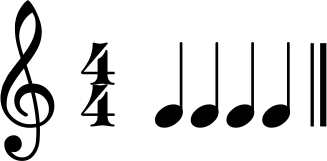
\includegraphics[scale=0.3]{img/discuss1}\\
\hline
\end{tabular}
}
}
\end{figure}

\begin{figure}[b!]
\subfloat[]{
\parbox{0.5\linewidth}{
\Tree
[ .{$\frac{1}{1}$} [ .{$\frac{1}{2}$} [ .{$\frac{1}{4}$} [ .$*$ ] [ .$\bullet$ ] ] [ .{$\frac{1}{4}$} [ .$\bullet$ ] [ .$\bullet$ ] ] ] [ .$\bullet$ ] ] 
}
}
\qquad
\subfloat[]{
\parbox{0.5\linewidth}{
\begin{tabular}{| l  >{\centering\arraybackslash}m{2in} |}
\hline 
A & 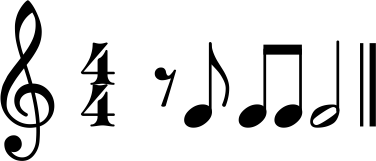
\includegraphics[scale=0.3]{img/discuss2}\\
B & 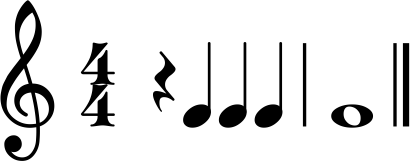
\includegraphics[scale=0.3]{img/discuss3}\\
\hline
\end{tabular}
}
}
\end{figure}

\begin{figure}[b!]
\parbox{0.5\linewidth}{
\subfloat[]{
\Tree
[ .{$\frac{1}{1}$} [ .{$\frac{1}{2}$} [ .{$\frac{1}{4}$} [ .$*$ ] [ .$\bullet$ ] ] [ .{$\frac{1}{4}$} [ .$\bullet$ ] [ .$\bullet$ ] ] ] [ .{$\frac{1}{2}$} [ .{$\frac{1}{4}$} [ .$\bullet$ ] [ .Rest ] ] [ .Rest ] ] ]
}
}
\qquad
\subfloat[]{
\parbox{0.5\linewidth}{
\begin{tabular}{| l  >{\centering\arraybackslash}m{2in} |}
\hline 
A & 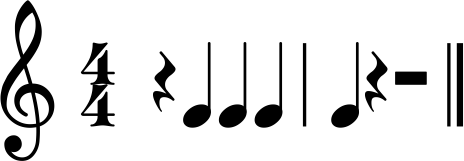
\includegraphics[scale=0.3]{img/discuss4}\\
\hline
\end{tabular}
}
}
\end{figure}

